% -----------------------------------------------------------------------------
% Implementation
% -----------------------------------------------------------------------------
\chapter{Implementation}

As noted before the ANC system has solely been implemented in the simulation environment Matlab. The system consist of several subsystems. These subsystems will be elaborated step by step and their functioning will be demonstrated.\\
The complete source code can be found in the \color{blue}\href{https://github.com/leonardberresheim/MA---Active-Noise-Control-in-Spatial-Domains/tree/main/Matlab}{projects github repository} \color{black} and is free to use, change and share without restrictions.



\section{Spherical Harmonics Decomposition}
The accuracy of the spherical harmonics decomposition in (\ref{eq:primary_noise_field}) with its truncation degree will be demonstrated using a plane wave \textit{(see figure \ref{fig:planeWaveExp}}) as the exact harmonic coefficients can be calculated using (\ref{eq:plane_wave_coefficients}).

\begin{figure}[H]
    \centerline{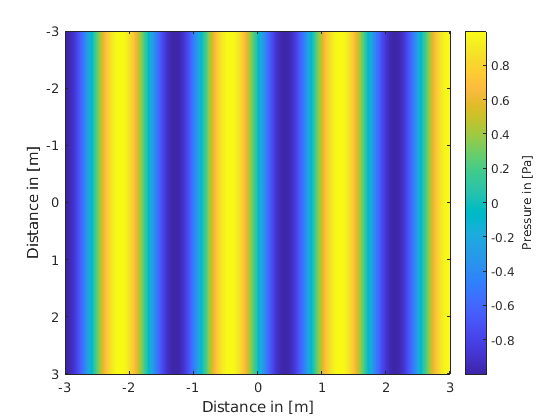
\includegraphics[width=100mm,keepaspectratio]{LaTeX/images/plots/plane_Wave_exponent_form.png}}
    \caption{Plane wave in exponent form.}
    \label{fig:planeWaveExp}
\end{figure}

\begin{figure}[H]
    \centerline{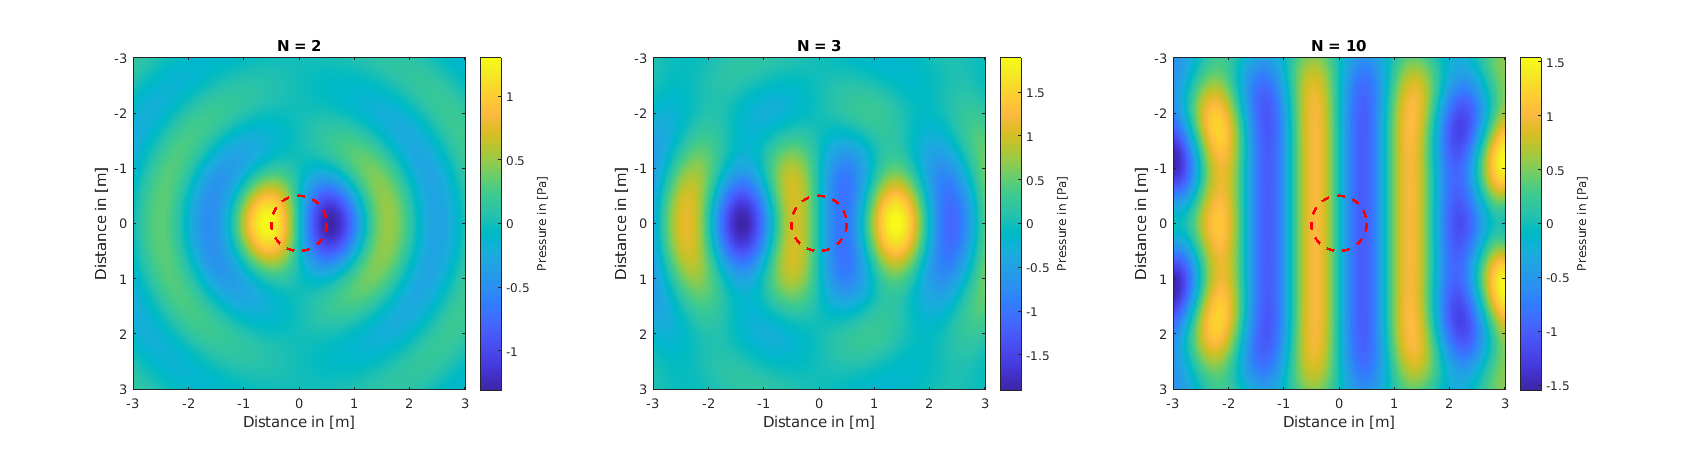
\includegraphics[width=180mm,keepaspectratio]{LaTeX/images/plots/Plane_wave_harmonics_form.png}}
    \caption{Plane wave in harmonics form for number of modes 2, 3 and 10}
    \label{fig:planeWaveHarmonics}
\end{figure}

When increasing the number of modes the resulting noise field gets closer and closer to the original plane wave in \textit{figure \ref{fig:planeWaveExp}} as can be seen in \textit{figure \ref{fig:planeWaveHarmonics}}. However only the quiet zone (\textit{marked as a red circle}) is of interest and with a higher number of modes the number of required loudspeakers increase as well as the computation time. In fact \textit{figure \ref{fig:planeWaveHarmonicsError}} shows that in the region of interest the accuracy of the spherical harmonics decomposition for $N = 3$ is already adequate.
\begin{figure}[H]
    \centerline{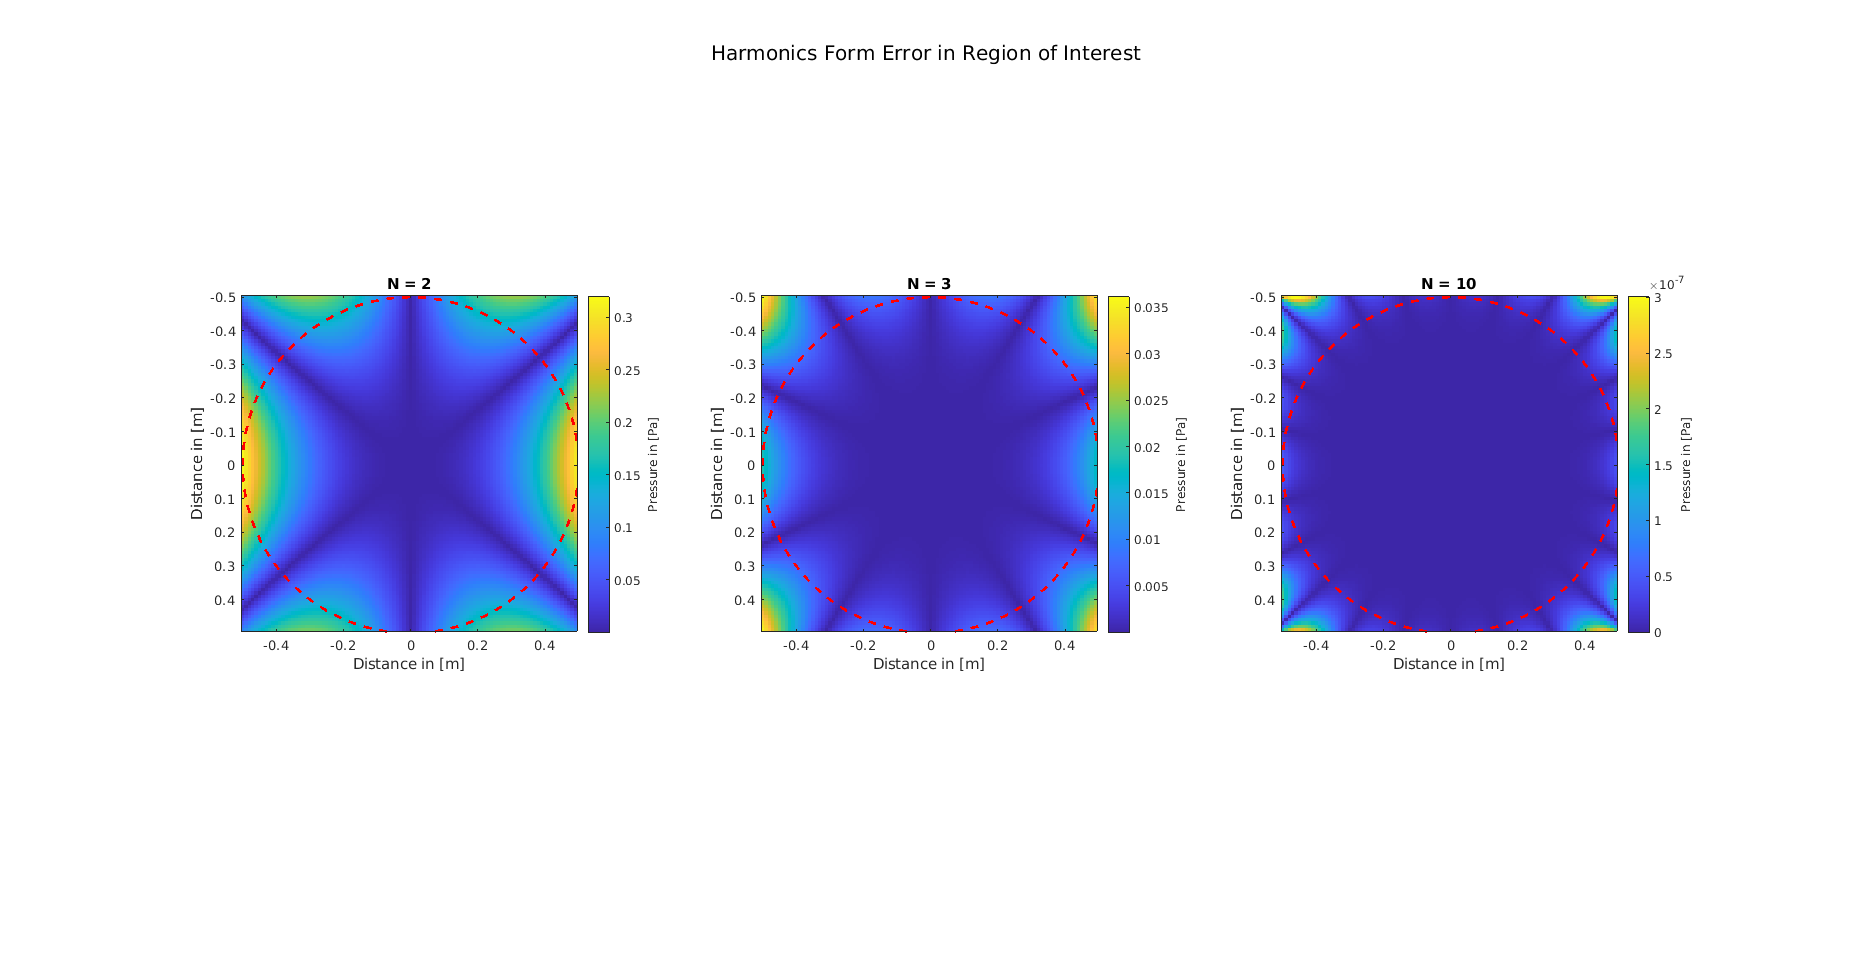
\includegraphics[width=180mm,keepaspectratio]{LaTeX/images/plots/Plane_wave_harmonics_form_Error.png}}
    \caption{Error of the plane wave in harmonics form within region of interest for number of modes 2, 3 and 10}
    \label{fig:planeWaveHarmonicsError}
\end{figure}
\\
\\
\textit{Nota}\\
Only the imaginary part is plotted here as the behavior of the real part of the wave is analogous to the imaginary part.
\section{Spherical Microphone Array}\label{sec:ImplSphMic}
The spherical microphone array is setup around the region of interest according to the Gaussian sampling scheme discussed in \textit{section \ref{sec:Gaussian}} with $2(N+1) = 8$ microphones on the azimuth angle in line with (\ref{eq:azimuth_sample}) and $(N + 1) = 4$ microphones on the elevation angle in line with (\ref{eq:elevation_sample}) resulting in a total of $2(N + 1)^2 = 32$ microphones arranged on the sphere \textit{(see figure \ref{fig:MicrophoneArray}})
\begin{figure}[H]
    \centerline{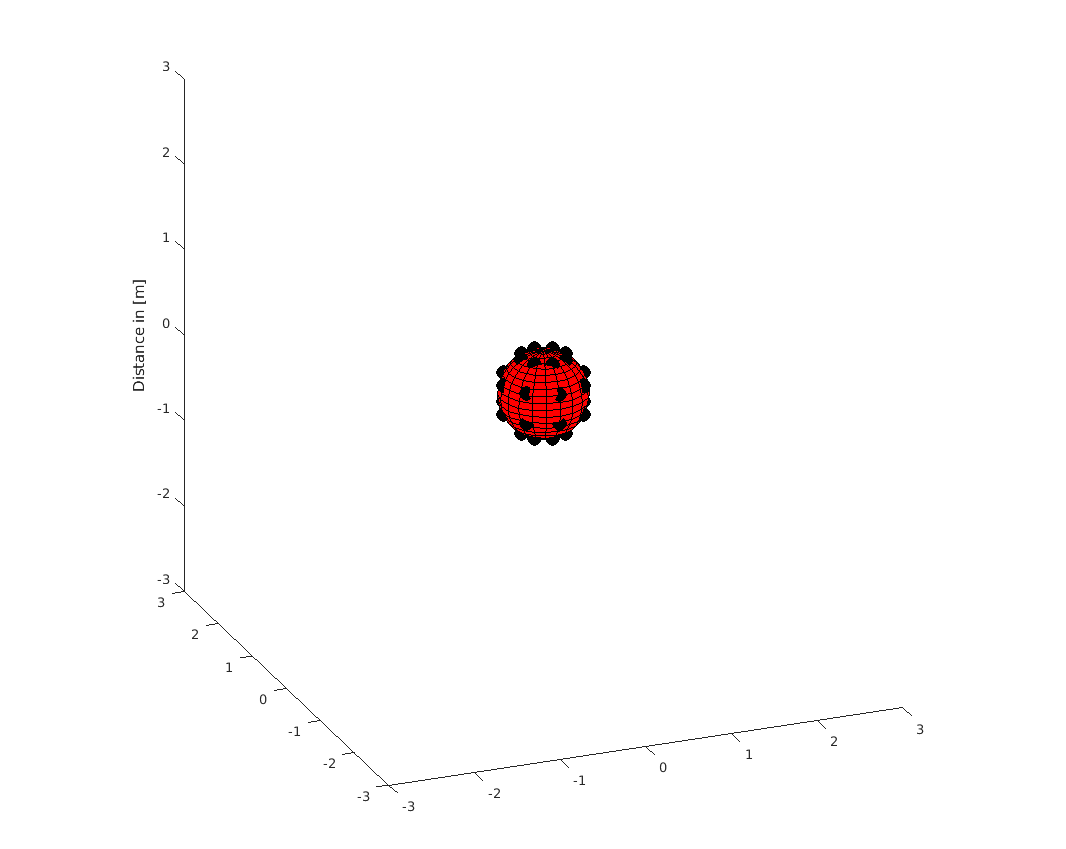
\includegraphics[width=180mm,keepaspectratio]{LaTeX/images/plots/MicrophoneArray.png}}
    \caption{Spherical microphone array arranged according to the Gaussian sampling scheme}
    \label{fig:MicrophoneArray}
\end{figure}
\section{Approximation of Harmonic Coefficient}
Applying the Gaussian sampling scheme discussed in \textit{section \ref{sec:Gaussian}}, the sampling weights are set according to (\ref{eq:gauss_weights}) and the harmonic coefficients for the noise field generated by the plane wave are approximated using (\ref{eq:gauss_harmonic_coefficients}).


\begin{figure}[H]
    \centerline{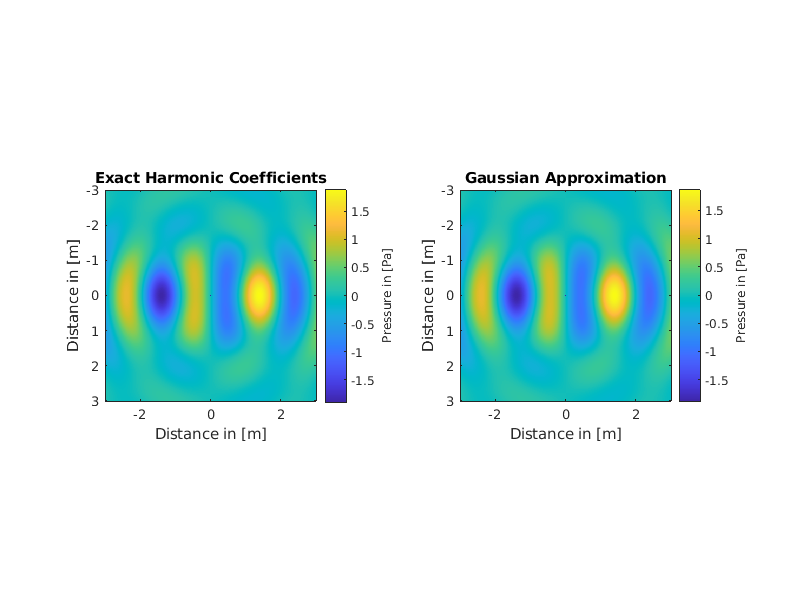
\includegraphics[width=180mm,keepaspectratio]{LaTeX/images/plots/Gauss_Approximation.png}}
    \caption{Plane wave noise field approximation in the wave domain with exact harmonic coefficients and Gaussian sampling approximation for N = 3}
    \label{fig:GaussianApproximation}
\end{figure}


The resulting noise field approximation using the Gaussian sampling scheme appears very similar to the exact noise field approximation\textit{(see figure \ref{fig:GaussianApproximation})}.\\
Surprisingly the error of the Gaussian approximation in regards to the actual plane wave is less at the corners than for the exact approximation as can be seen in \textit{figure \ref{fig:GaussianApproximationError}}.\\\\

\textit{Nota}\\
By \textit{exact} the analytical solution to the harmonic coefficient from (\ref{eq:plane_wave_coefficients}) in consideration of the truncation order of $N = 3$ is meant. 


\begin{figure}[H]
    \centerline{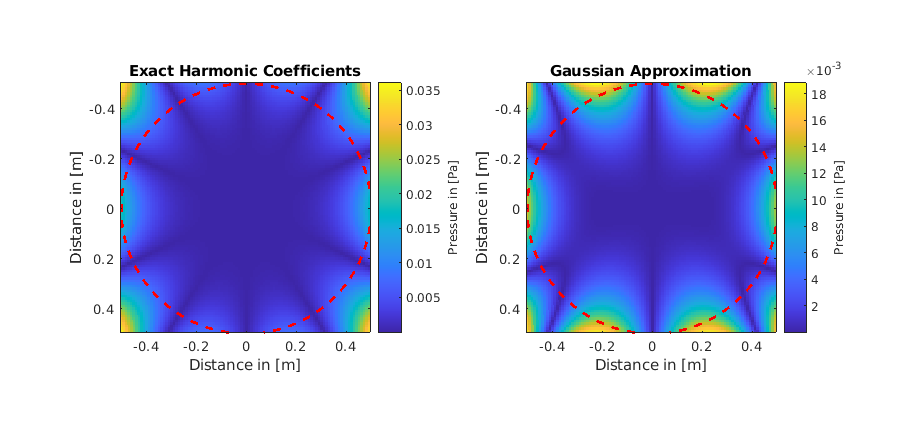
\includegraphics[width=180mm,keepaspectratio]{LaTeX/images/plots/Gauss_Approximation_Error.png}}
    \caption{Error for the plane wave noise field approximation in the wave domain with exact harmonic coefficients and Gaussian sampling approximation for N = 3}
    \label{fig:GaussianApproximationError}
\end{figure}

\section{Simulation Setup}
The simulation setup is set in accordance with \cite{Zhang2019}. The environment is modeled by a \textit{shoebox} room of $6m \times 6m \times 5m$ with reflection coefficients set to $[0.75,0.8,0.77,0.85,0.1,0.1]$ usual for a common room with relatively high reflection coefficients for the walls and relatively low reflection coefficients for floor and ceiling. The source is modeled as a point source as defined by (\ref{eq:point_source}). For now we assume the noise field to contain only a single frequency component of $200Hz$ and the point source to emit at a constant magnitude of 10.\\ \\
The region of interest is a spherical area of radius $R_1 = 0.5m$ located at the origin which as seen in \textit{section \ref{sec:primary}} leads to a number of modes of $N = \lceil ekR_1/2\rceil = 3$. As depicted in \textit{section \ref{sec:matching}} $(N+1)^2 = 16$ loudspeakers would be necessary to bear an exact solution. But as aforementioned and discussed \textit{Case 3} will be realized in which the number of loudspeakers is lesser and thus an approximation is required. The source is located at $(2, 315^\circ , 90^\circ)$ and the number of loudspeaker is set to 12 and arranged as seen in \textit{figure \ref{fig:setup}}.

\begin{figure}
    \centerline{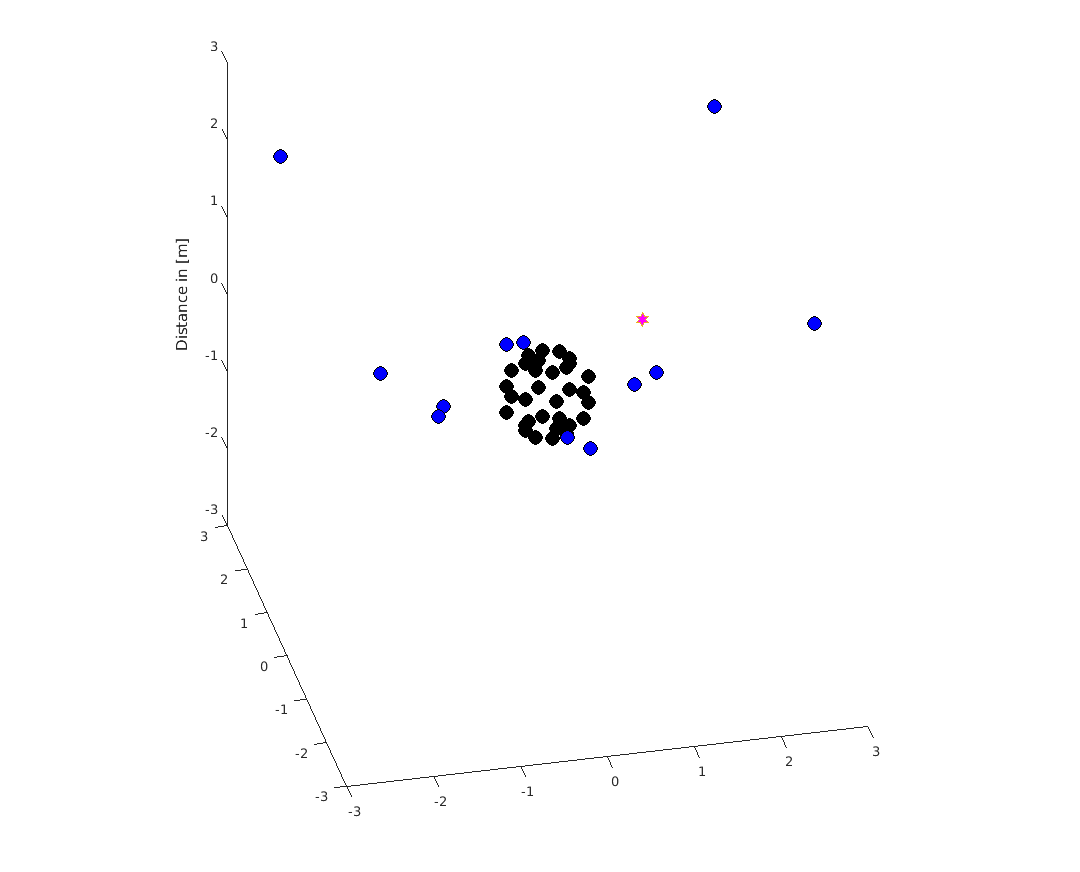
\includegraphics[width=180mm,keepaspectratio]{LaTeX/images/plots/ANCSetup.png}}
    \caption{Simulation setup, where the blue points are the loudspeakers positions, the pink star is the noise source position and the black points represent the microphones positions}
    \label{fig:setup}
\end{figure}
\newpage

\section{Point Source Reverberation}
\textit{Figure \ref{fig:reverberation}} depicts the primary noise field emitted by the point source and its reverberation in the room caused by the walls reflection before any interference of the active noise cancelling system. The objective is to have the sound energy within the region of interest \textit{(red circle)} to be reduced to a minimum.

\begin{figure}[H]
    \centerline{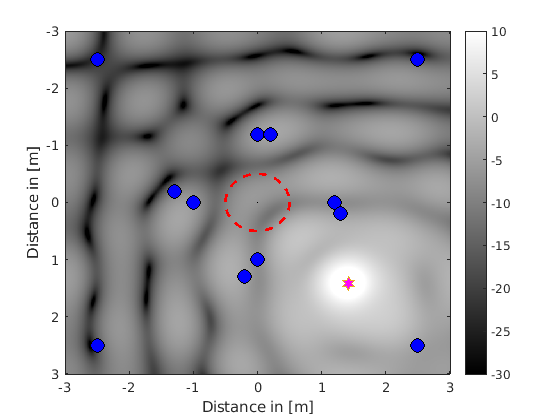
\includegraphics[width=\textwidth]{LaTeX/images/plots/Point_source_reverberation.png}}
    \caption{Sound energy of primary noise field emitted by a point source and its reverberation in the room caused by the walls reflection with projection of loudspeakers and region of interest on the x-y-plane}
    \label{fig:reverberation}
\end{figure}

\section{Active Noise Control}
The same steps as in \textit{section \ref{sec:ImplSphMic}} are taken to determine the approximation of the harmonic coefficients for the primary noise field in the region of interest.\\
The process is repeated analogously to compute the harmonic coefficients for the acoustic transfer function in (\ref{eq:ATF_wavedomain}) applying the image source method discussed in \textit{section \ref{sec:ism}}.\\
The harmonic coefficients for the primary noise field and the coefficients for the acoustic transfer function are put into vector form in accordance with (\ref{eq:primary_coefs_vector}) and (\ref{eq:secondary_coef_vector}) respectively.\\
The loudspeakers driving signals can then be resolved using (\ref{eq:matching}).
The secondary noise field can now be calculated applying the loudspeakers driving signals and the acoustic transfer function in to (\ref{eq:secondary_noise_field_atf}).\\\\
Adding the secondary noise field to the primary noise field as in (\ref{eq:residual}) results in the residual noise as pictured in \textit{figure \ref{fig:ANC1}}. As intended the noise field emitted by the loudspeakers results in a satisfactory reduction of the sound energy within the region of interest. It can thus be claimed to have successfully implemented a \textit{spatial ANC} system for a given setup in a simulation environment.\\\\

\begin{figure}[H]
    \centerline{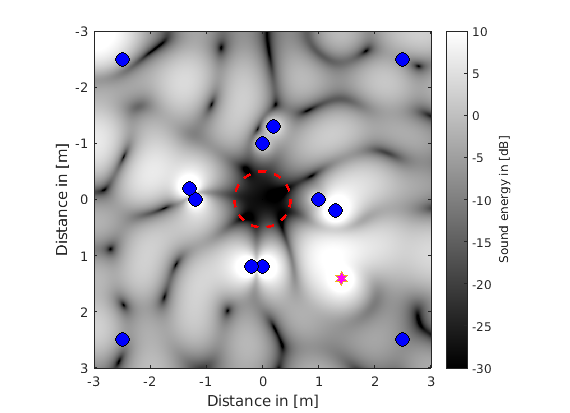
\includegraphics[width=\textwidth]{LaTeX/images/plots/ANC_1.png}}
    \caption{Sound Energy of residual noise field}
    \label{fig:ANC1}
\end{figure}

To test the stability of the system the process is repeated with different positions for the noise source.\\
The results show that in each case a quiet zone is created in the region of interrest, unfortunately this zone is only relatively quiet in comparison to the noise emitted by the loudspeakers. When comparing it to the residual noise before the impact of the ANC system, only for the tests resulting in \textit{figure \ref{fig:ANC3}} and \textit{\ref{fig:ANC4}} there is a slight improvement within the quiet zone. Additionally as seen in \textit{figure \ref{fig:ANC2}} and \textit{\ref{fig:ANC3}} the residual noise outside the region of interest is highly intensified which in certain environments could be problematic.
\begin{figure}[H]
    \centerline{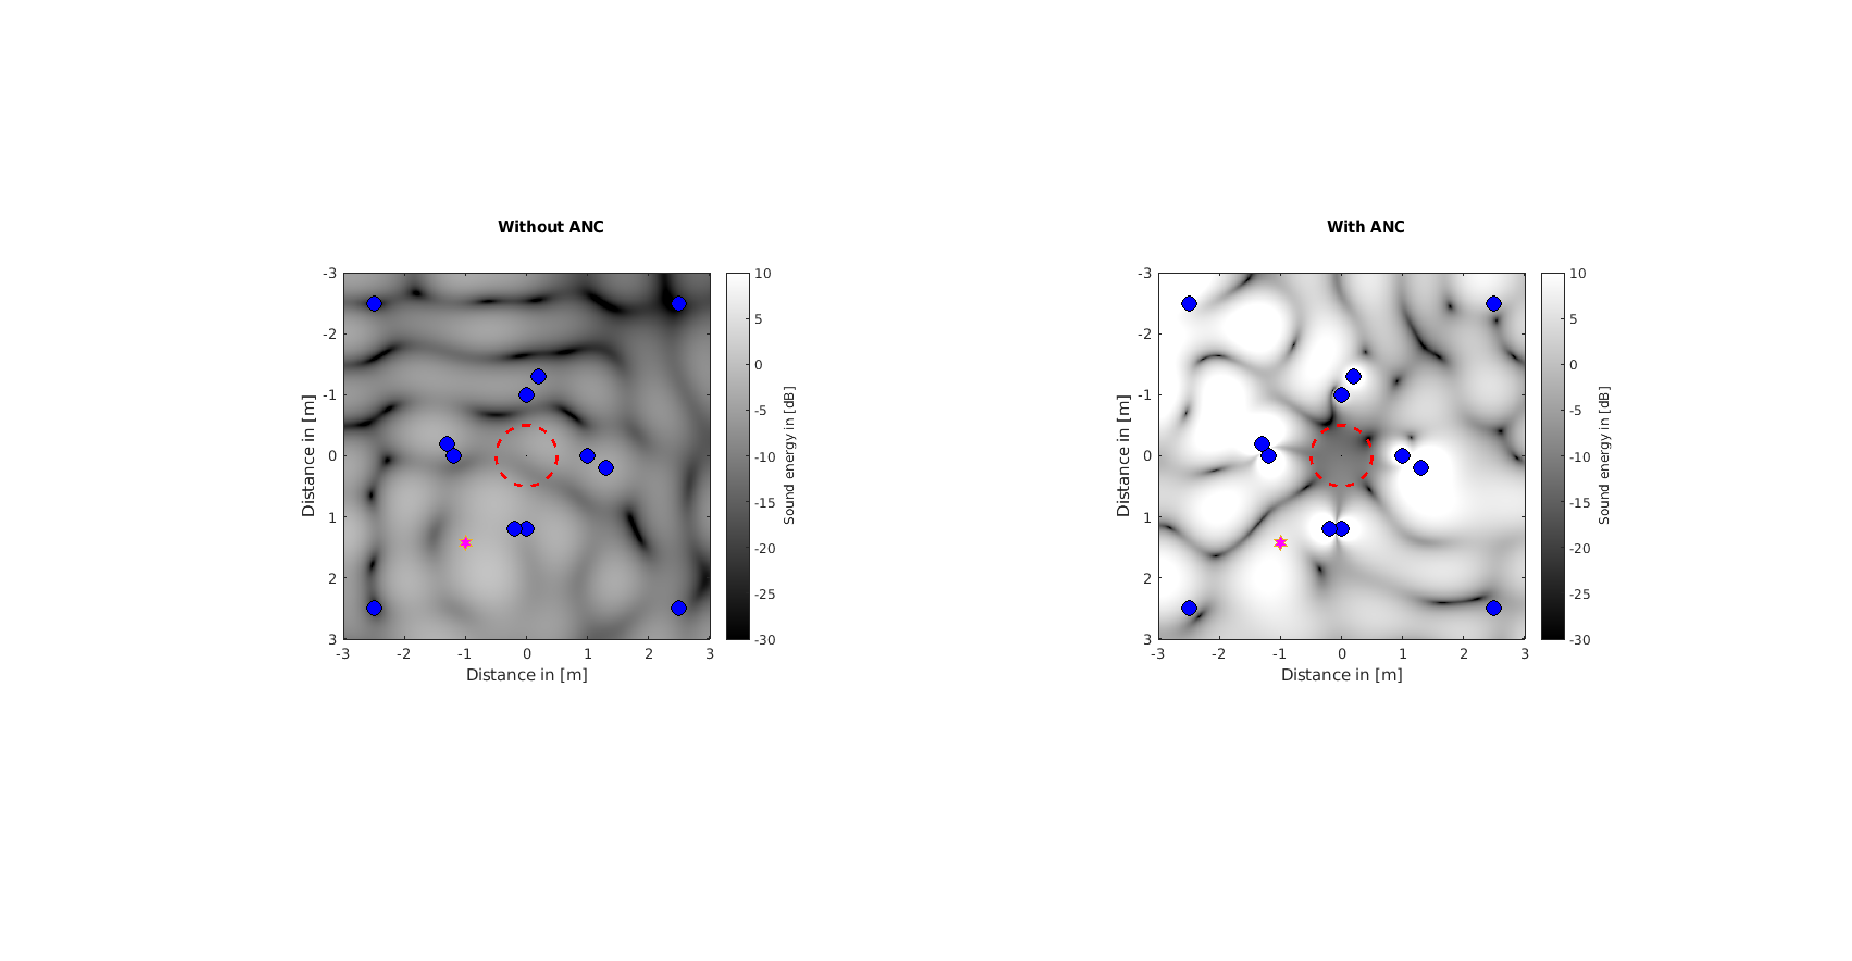
\includegraphics[width=180mm,keepaspectratio]{LaTeX/images/plots/ANC_2_both.png}}
    \caption{Residual noise with and without ANC for source located at $(2, 305◦ , 120◦)$}
    \label{fig:ANC2}
\end{figure}
\begin{figure}[H]
    \centerline{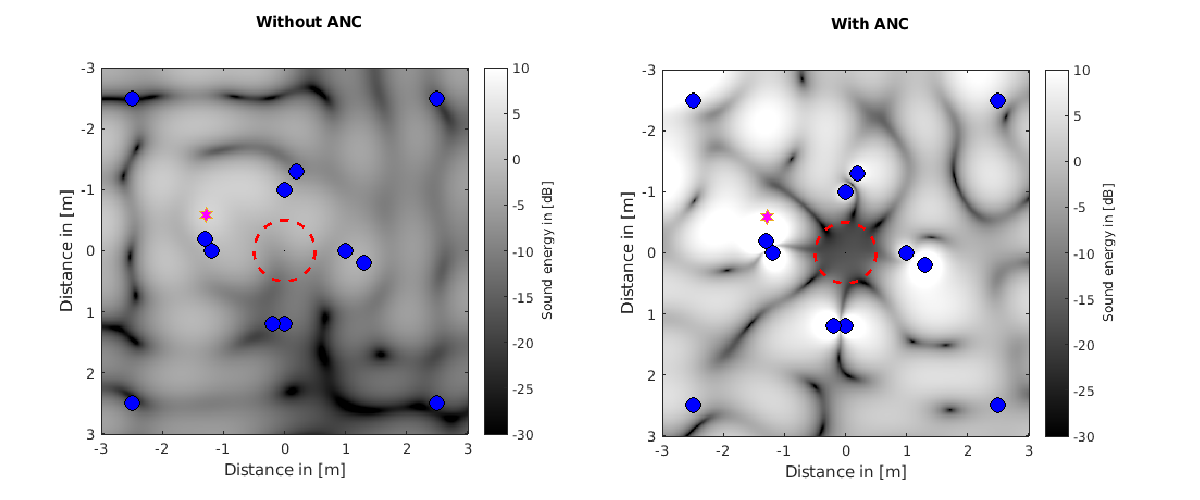
\includegraphics[width=180mm,keepaspectratio]{LaTeX/images/plots/ANC_3_both.png}}
    \caption{Residual noise with and without ANC for source located at $(1.5, 205◦ , 70◦)$}
    \label{fig:ANC3}
\end{figure}
\begin{figure}[H]
    \centerline{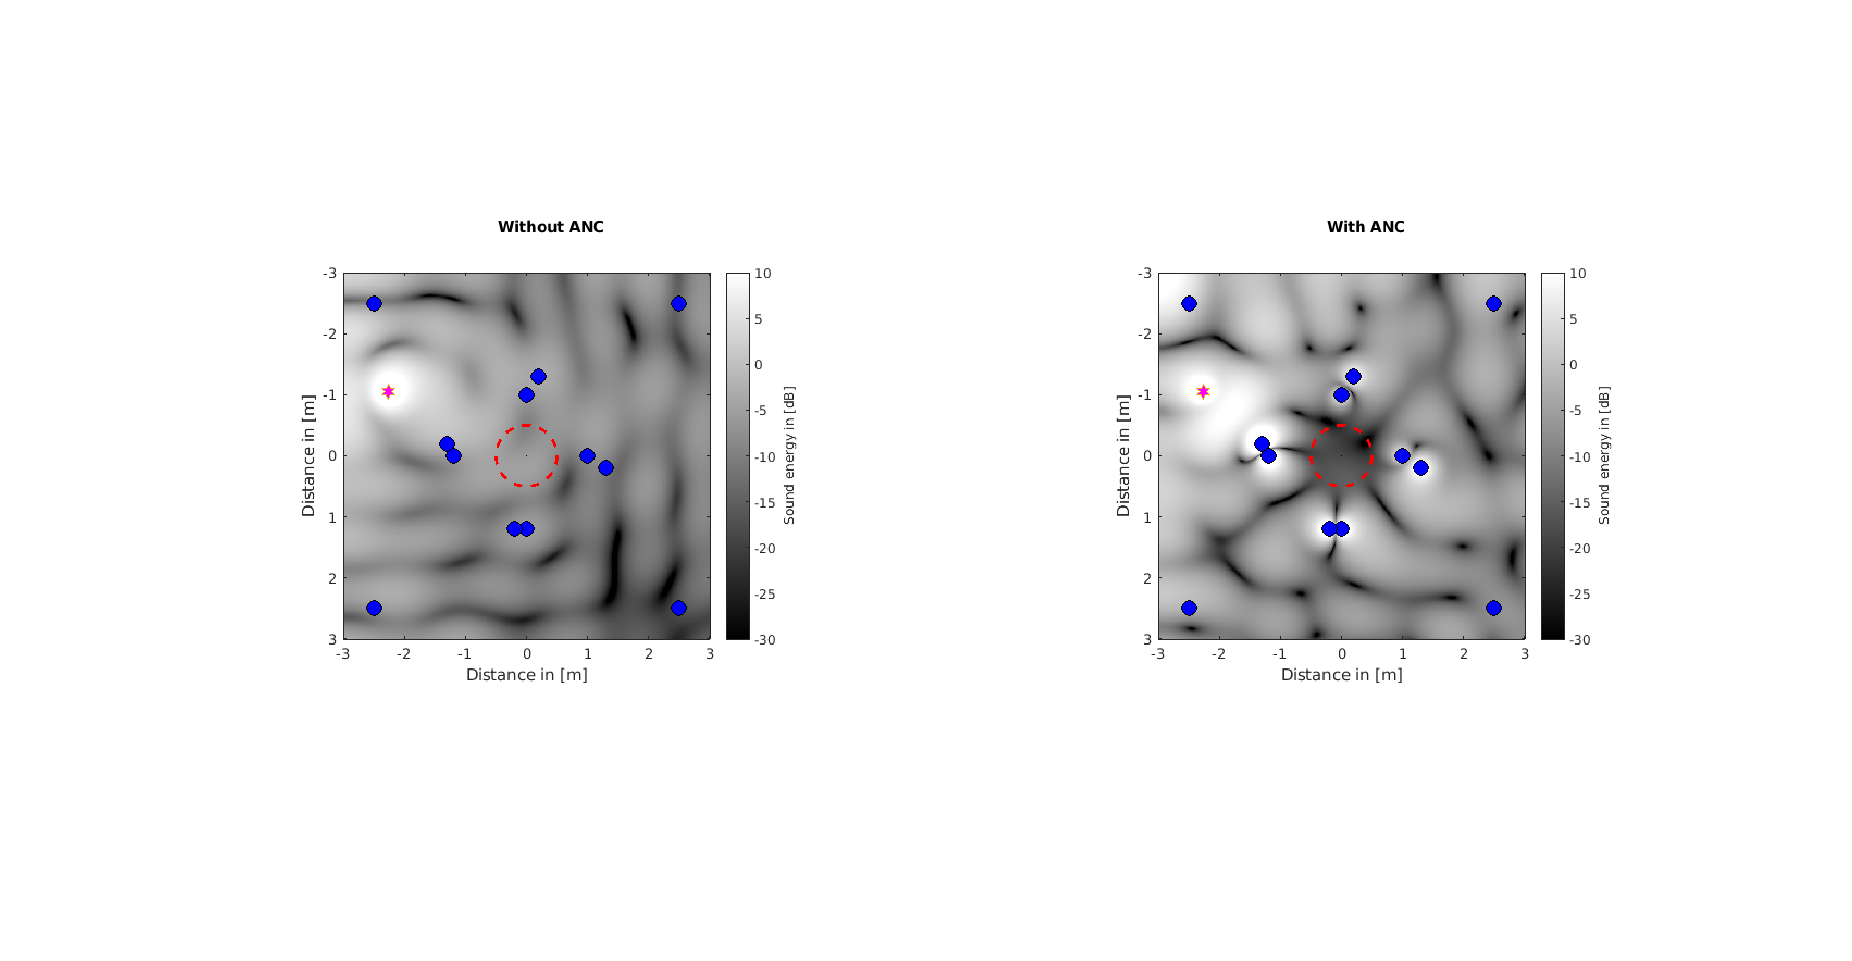
\includegraphics[width=180mm,keepaspectratio]{LaTeX/images/plots/ANC_4_both.png}}
    \caption{Residual noise with and without ANC for source located at $(2.5, 205◦ , 90◦)$}
    \label{fig:ANC4}
\end{figure}

